
\begin{enumerate}[label=\thesubsection.\arabic*.,ref=\thesubsection.\theenumi]
\numberwithin{equation}{enumi}
\item Given the unity feedback system, with
\begin{align}
G(S) = \frac{K(s+10)(s+11)}{s(s+3)(s+6)(s+9)}
\end{align}
Use frequency response method to design a lag compensator to yield Kv = 1000 and peak overshoot of 15\% .Use second order approximation. \\
%
\solution Fig. \ref{fig:ee18btech11030_block} models the equivalent of compensated closed loop system. 
\begin{figure}[!ht]
\begin{center}
	\resizebox{\columnwidth}{!}{ 
\usetikzlibrary{decorations.markings}
\begin{circuitikz}
\draw (-4,-1) to[amp,t={+K}] (2.5,-1);
\draw (-4,-1) to (-4,2) to (-3,2) ;
\draw (-3,2)  to [capacitor=$C/10$](-3,0.5) to  (-3,0.5) node[ground]{};
\draw (-3,2) to (-2.3,2)to [R=$10R$] (-1.3,2)to (0,2) to [R=$R$] (0,5) node[label={}]{}  to (-4,5) ;
\draw (0,2) to(1,2) to  [capacitor=$C$](1.5,2) to (2.5,2) to (2.5,-1);
\draw (-4,5) to (-4,4.7) to [V=$V_s$] (-4,3.9) to (-4,3.5) node[ground]{} ;
\draw (2.5,-1) to[short, -o] (3,-1) node[label={above:$V_{out}$}]{};
\end{circuitikz}}
\end{center}
\caption{}
\label{fig:ee18btech11030_block}
\end{figure}

%

Velocity constant  
\begin{align}
K_{v} =  \lim_{t \to 0}sG(s)
\end{align}
\begin{align}
\lim_{t \to 0}s\frac{K(s+10)(s+11)}{s(s+3)(s+6)(s+9)} &= 1000
\end{align}
\begin{align}
\implies K &= 1473
\end{align}
Bode plot of G(s) for the value of k
%
\begin{figure}[!ht]
\centering
  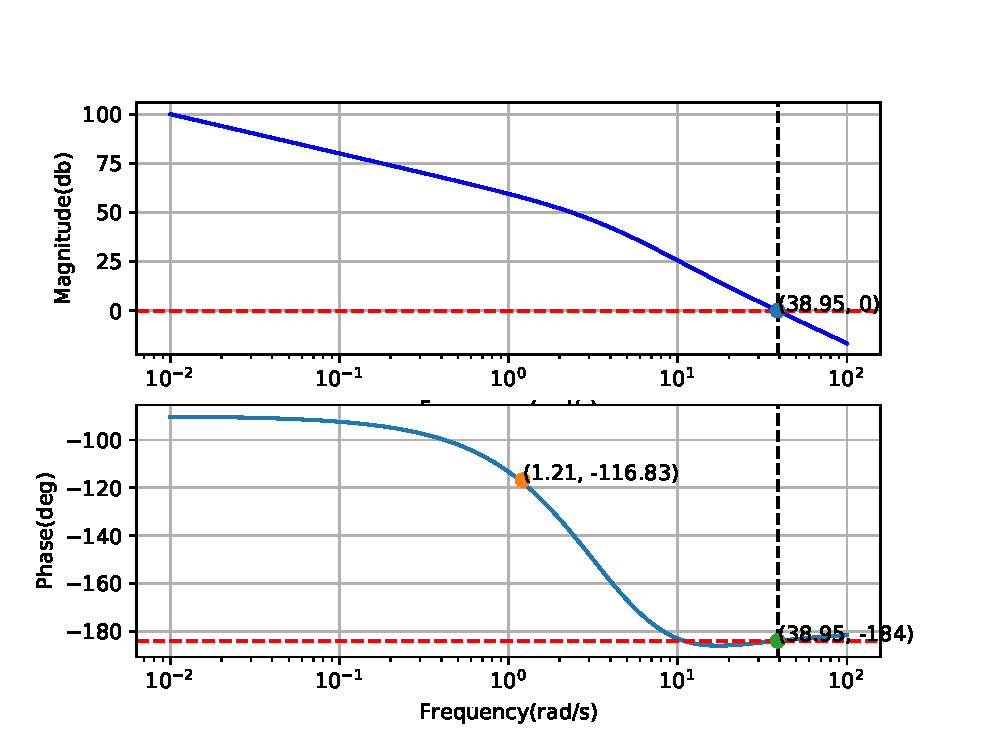
\includegraphics[width=\columnwidth]{./figs/ee18btech11030/ee18btech11030_1.eps}
\caption{}
\label{fig:ee18btech11030_1}
\end{figure}

The following code verifies the result.
\begin{lstlisting}
codes/ee18btech11030/ee18btech11030.py
\end{lstlisting}
%

Relation between \%OS and Damping ratio
\begin{align}
\zeta &= \frac{-\ln(\%OS/100)}{\sqrt{(\pi)^2 + (\ln(\%OS/100))^2}}
\end{align}
\begin{align}
\implies\zeta &= 0.517 
\end{align}
Phase Margin for a Damping ratio is given by Eq \eqref{eq:ee18btech11030}  
\begin{align}
\label{eq:ee18btech11030}
\phi_{m} &= 90\degree - \arctan(\frac{\sqrt{-2\zeta^2+\sqrt{1+4\zeta^4}}}{2\zeta}
\end{align}
\begin{align}
\implies \phi_{m} &= 53.17\degree
\end{align}

From Fig : \ref{fig:ee18btech11030_1} of uncompensated system with K = 1473 
\begin{align}
\phi_{m} = -4\degree \text{, } \omega_{PM} &= 38.95 rad/sec
\end{align}
\begin{align}
\phi_{ml}\text{ lies in (5,12)}
\end{align}
\begin{align}
     \phi_{total} & = 53.17\degree  -(-4\degree ) + \phi{ml}
\end{align}
\begin{align}
    \phi_{total} &= 63.17\degree
\end{align}
\textbf{Note} : Adding 6 degrees phase angle to compensate the phase angle contribution of the lag compensator.

From Figure \ref{fig:ee18btech11030_1} 
\begin{align}
     \phi_{total} & = 63.17\degree \text{ at, } \omega_{PM} &= 1.21 rad/sec
\end{align}
At this Phase Margin frequency, the magnitude plot must go through 0 dB. But The magnitude of uncompensated system at 1.21 rad/sec is 57.55 dB = 754.2  

\item Designing Lag Compensator Gc(s)
\\
\solution 
General lag compensator 
\begin{align}
G_{c}(s) &= \left(\frac{s+\frac{1}{T}}{s+\frac{1}{T\alpha}}\right)  \text{  } \alpha > 1
\end{align}
\begin{itemize}
\item First draw the high-frequency asymptote at -57.55 dB.So that magnitude at 1.21 rad/sec becomes 0 dB.
\item Arbitrarily select the higher break frequency to be about one decade below the phase-margin frequency, or 0.121 rad/sec.
\item Starting at the intersection of this frequency with the lag compensator’s high-frequency asymptote, draw a
-20 dB/decade line until 0 dB is reached.That intersection gives the lower break frequency.
\item The lower break frequency is found to be 0.0001604 rad/sec. 
\item The compensator must have a dc gain of unity to retain the value of Kv that we have already designed by setting K = 1473. 

\item Gain in the lag compensator = 0.001326

\end{itemize}
\begin{align}
 Gain &= \frac{0.0001604}{0.121} = 0.001326 
\end{align}

Hence the lag compensator transfer function is
\begin{align}
 G_{c}(s) &= \frac{0.001326(s+0.121)}{s+0.0001604} 
\end{align}
\item Verifying Lag Compensator using Plots
\\
\solution Magnitude and Phase plot


\begin{figure}[!ht]
\centering
  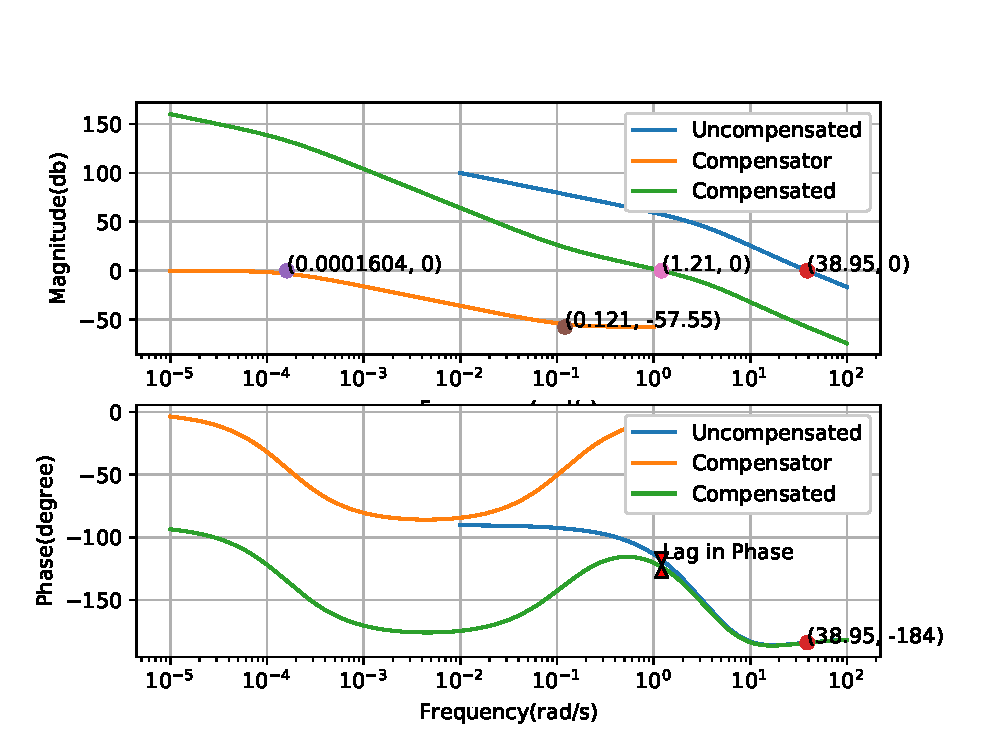
\includegraphics[width=\columnwidth]{./figs/ee18btech11030/ee18btech11030_2.eps}
\caption{} 
\label{fig:ee18btech11030_2}
\end{figure}


The following code 
\begin{lstlisting}
codes/ee18btech11030/ee18btech11030_1.py
\end{lstlisting}


\begin{table}[!ht]
\centering
 
\usetikzlibrary{decorations.markings}
\begin{circuitikz}
\draw (-4,-1) to[amp,t={+K}] (2.5,-1);
\draw (-4,-1) to (-4,2) to (-3,2) ;
\draw (-3,2)  to [capacitor=$C/10$](-3,0.5) to  (-3,0.5) node[ground]{};
\draw (-3,2) to (-2.3,2)to [R=$10R$] (-1.3,2)to (0,2) to [R=$R$] (0,5) node[label={}]{}  to (-4,5) ;
\draw (0,2) to(1,2) to  [capacitor=$C$](1.5,2) to (2.5,2) to (2.5,-1);
\draw (-4,5) to (-4,4.7) to [V=$V_s$] (-4,3.9) to (-4,3.5) node[ground]{} ;
\draw (2.5,-1) to[short, -o] (3,-1) node[label={above:$V_{out}$}]{};
\end{circuitikz}
\caption{Comparing the Proposed and Actual results}
\label{table:ee18btech11030_table}
\end{table}

\item Verifying in time domain 
\\
\solution 
Time response for a unit step function

\begin{figure}[!ht]
\centering
  \includegraphics[width=\columnwidth]{./figs/ee18btech11030/ee18btech11030_3.eps}
\caption{}
\label{fig:ee18btech11030_3} 
\end{figure}

The following code 
\begin{lstlisting}
codes/ee18btech11030/ee18btech11030_2.py
\end{lstlisting}

\end{enumerate}
